\documentclass[tikz,border=8pt]{standalone}
% Shared look for every TikZ diagram. Load with \input{../../tools/tikz-style.tex}
\usepackage[sfdefault]{roboto}
\usetikzlibrary{arrows.meta, positioning, shapes.geometric, calc, fit, backgrounds}
\definecolor{cblue}{HTML}{4C78A8}
\definecolor{corange}{HTML}{F58518}
\definecolor{cgreen}{HTML}{54A24B}
\definecolor{cred}{HTML}{E45756}
\definecolor{cpurple}{HTML}{B279A2}
\definecolor{cgrey}{HTML}{6B6B6B}
\tikzset{
  every picture/.style={font=\sffamily, line width=1.2pt},
  box/.style={draw=#1, fill=#1!12, rounded corners=4pt, align=center, inner sep=7pt, minimum height=1.1cm},
  box/.default=cgrey,
  arrow/.style={-{Stealth[length=3mm]}, draw=cgrey, line width=1.4pt},
  title/.style={font=\sffamily\bfseries\Large},
  note/.style={font=\sffamily\small, text=cgrey, align=center},
}
\AtBeginDocument{\hyphenpenalty=10000 \exhyphenpenalty=10000}

% Nav2 (ros-navigation/navigation2, main): nav2_bringup/launch/bringup_launch.py includes localization_launch.py
% (map_server, amcl), keepout_zone_launch.py and speed_zone_launch.py (two filter servers each, both on by default) and
% navigation_launch.py (11 servers), and starts one lifecycle manager, lifecycle_manager_nav2, whose node_names list
% holds those 17 lifecycle nodes. Autoware (autowarefoundation/autoware_launch, main):
% autoware_launch/launch/autoware.launch.xml includes one launch file per component, each behind a launch_* switch.
\begin{document}
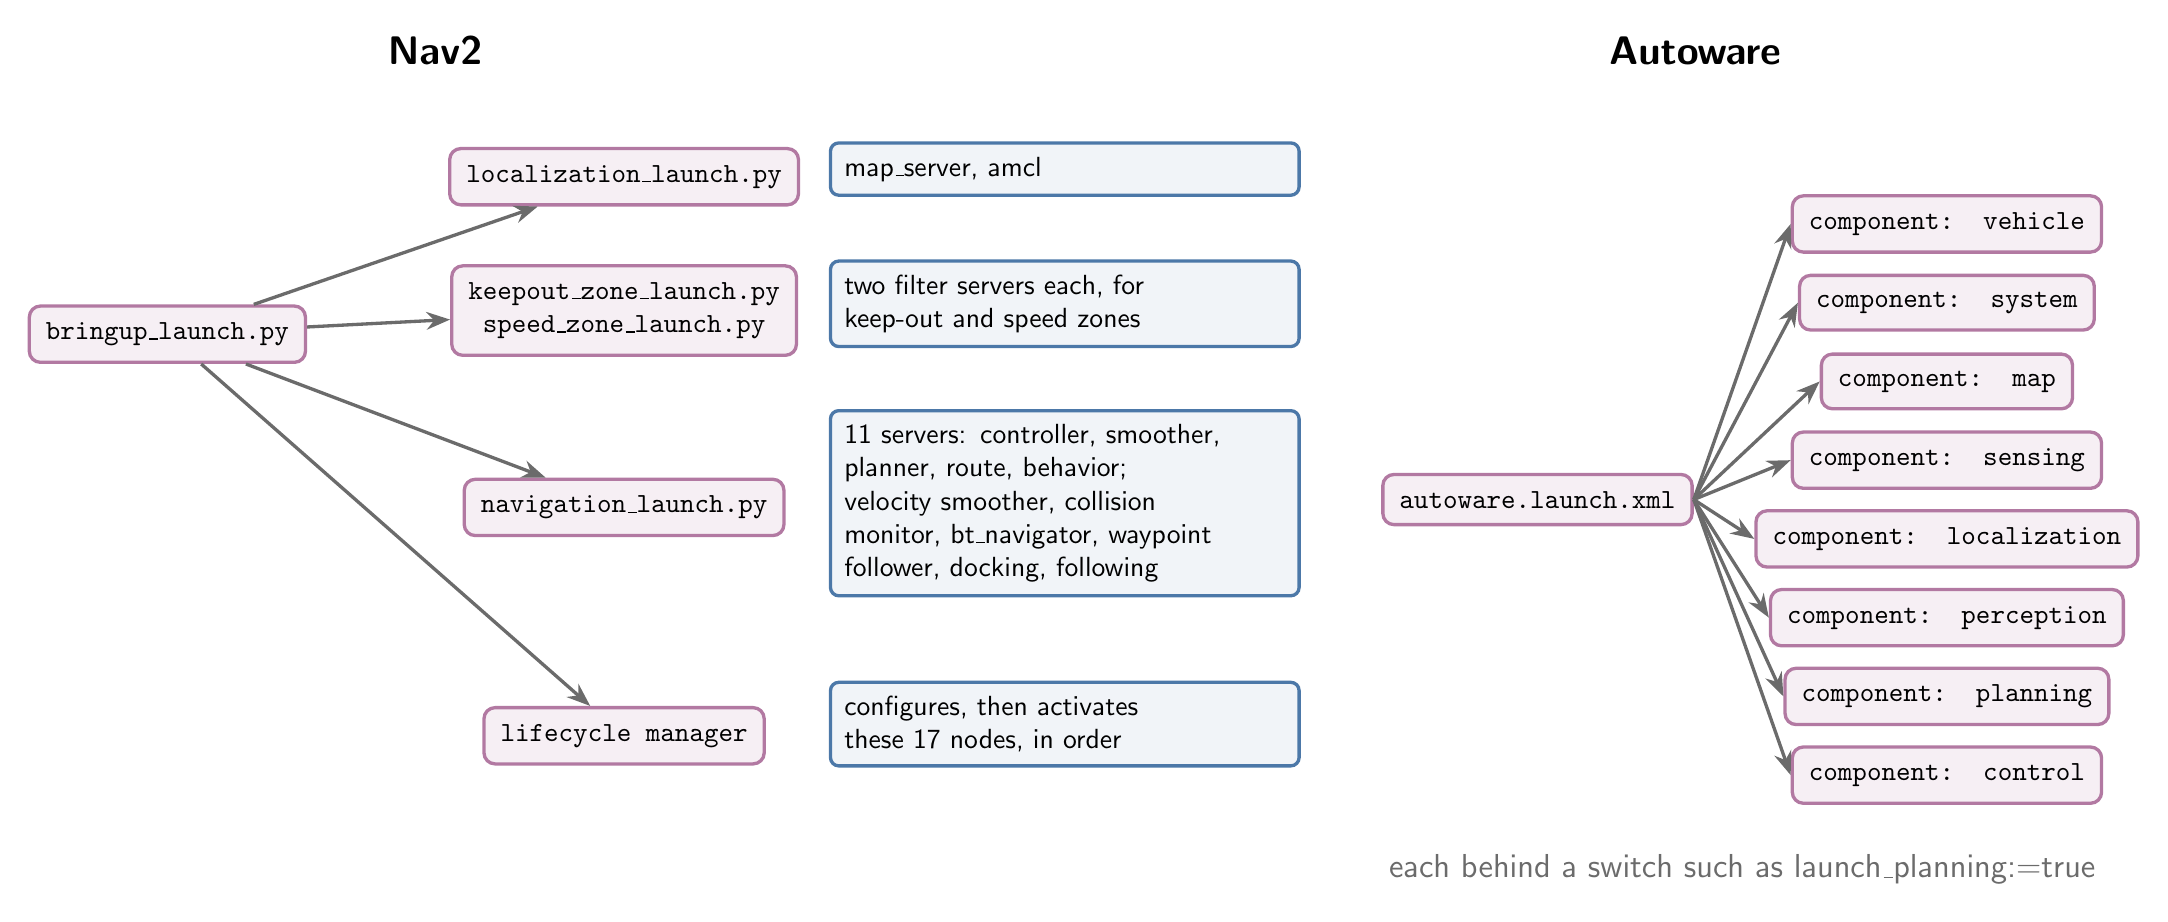
\begin{tikzpicture}[
  lf/.style={draw=cpurple, fill=cpurple!12, rounded corners=4pt, font=\ttfamily\normalsize, align=center, inner sep=6pt},
  nl/.style={draw=cblue, fill=cblue!8, rounded corners=3pt, font=\sffamily\normalsize, align=left, inner sep=5pt, text width=5.6cm},
  ar/.style={-{Stealth[length=3mm]}, draw=cgrey, line width=1.2pt}]
  \node[title] at (3.4,7.2) {Nav2};
  \node[lf] (b) at (0,3.6) {bringup\_launch.py};
  \node[lf] (l) at (5.8,5.6) {localization\_launch.py};
  \node[lf] (z) at (5.8,3.9) {keepout\_zone\_launch.py\\ speed\_zone\_launch.py};
  \node[lf] (n) at (5.8,1.4) {navigation\_launch.py};
  \node[lf] (m) at (5.8,-1.5) {lifecycle manager};
  \node[nl, anchor=north west] at (8.4,6.05) {map\_server, amcl};
  \node[nl, anchor=north west] at (8.4,4.55) {two filter servers each, for\\ keep-out and speed zones};
  \node[nl, anchor=north west] at (8.4,2.65) {11 servers: controller, smoother,\\ planner, route, behavior;\\ velocity smoother, collision\\ monitor, bt\_navigator, waypoint\\ follower, docking, following};
  \node[nl, anchor=north west] at (8.4,-0.8) {configures, then activates\\ these 17 nodes, in order};
  \draw[ar] (b) -- (l); \draw[ar] (b) -- (z); \draw[ar] (b) -- (n); \draw[ar] (b) -- (m);
  \node[title] at (19.4,7.2) {Autoware};
  \node[lf] (a) at (17.4,1.5) {autoware.launch.xml};
  \foreach \c/\y in {vehicle/5.0, system/4.0, map/3.0, sensing/2.0, localization/1.0, perception/0.0, planning/-1.0, control/-2.0}
    {\node[lf] (\c) at (22.6,\y) {component: \c}; \draw[ar] (a.east) -- (\c.west);}
  \node[note, font=\sffamily\large, align=center] at (20.0,-3.2) {each behind a switch such as launch\_planning:=true};
\end{tikzpicture}
\end{document}
